\documentclass[tikz,border=6pt]{standalone}
\usepackage{ctex}
\usepackage{amsmath}
\usetikzlibrary{arrows.meta,positioning,calc}

\begin{document}
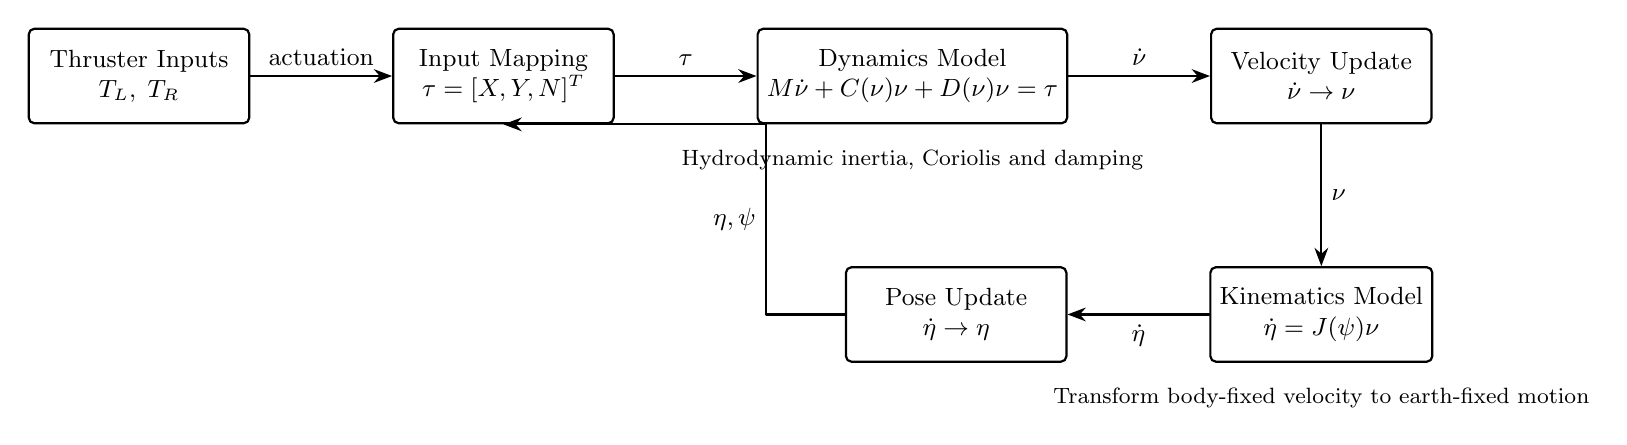
\begin{tikzpicture}[
    >=Stealth,
    font=\small,
    line join=round,
    line cap=round,
    block/.style={
        draw,
        thick,
        rectangle,
        rounded corners=2pt,
        minimum width=2.8cm,
        minimum height=1.2cm,
        align=center
    },
    signal/.style={->, thick},
    note/.style={font=\footnotesize, align=center}
]

% =========================
% Nodes
% =========================
\node[block] (thruster) {Thruster Inputs\\$T_L,\;T_R$};

\node[block, right=1.8cm of thruster] (mapping) {Input Mapping\\$\tau = [X,Y,N]^T$};

\node[block, right=1.8cm of mapping, minimum width=3.7cm] (dynamics) {Dynamics Model\\$M\dot{\nu}+C(\nu)\nu+D(\nu)\nu=\tau$};

\node[block, right=1.8cm of dynamics] (vel) {Velocity Update\\$\dot{\nu}\rightarrow \nu$};

\node[block, below=1.8cm of vel] (kinematics) {Kinematics Model\\$\dot{\eta}=J(\psi)\nu$};

\node[block, left=1.8cm of kinematics] (pose) {Pose Update\\$\dot{\eta}\rightarrow \eta$};

% =========================
% Main chain
% =========================
\draw[signal] (thruster) -- node[above] {actuation} (mapping);
\draw[signal] (mapping) -- node[above] {$\tau$} (dynamics);
\draw[signal] (dynamics) -- node[above] {$\dot{\nu}$} (vel);

\draw[signal] (vel) -- node[right] {$\nu$} (kinematics);
\draw[signal] (kinematics) -- node[below] {$\dot{\eta}$} (pose);

% =========================
% Optional feedback / state coupling
% =========================
\draw[signal] (pose.west) -- ++(-1.0,0) |- node[pos=0.25,left] {$\eta,\psi$} (mapping.south);

% =========================
% Notes
% =========================
\node[note, below=0.2cm of dynamics] {Hydrodynamic inertia, Coriolis and damping};
\node[note, below=0.2cm of kinematics] {Transform body-fixed velocity to earth-fixed motion};

\end{tikzpicture}
\end{document}